\section{Evaluation with Java Projects}
\label{sec:eval:java}

In this section, we evaluate the precision and recall of our approach using a recently proposed dataset of refactorings performed in real-world Java open source projects. We also compare RefDiff's accuracy with RMiner, 
a state-of-the-art tool for detecting refactorings in Java.
First, we present our evaluation design (Section~\ref{sec:eval:java:design}) and then we present the results (Section~\ref{sec:eval:java:results}).

\subsection{Evaluation Design}
\label{sec:eval:java:design}

To evaluate the precision and recall of RefDiff in Java we initially use an oracle proposed by Tsantalis et al.~\cite{tsantalis2018rminer}.
This oracle includes 3,188 manually-validated refactoring instances, detected in 538 commits from 185 open source projects, and covering 15 refactoring operations.
We also use this oracle to compare RefDiff's precision and recall against RMiner.
For the purpose of the comparison, we restricted the oracle to 11 refactoring types supported by both tools.
Specifically, we excluded \emph{Change Package}, \emph{Move Field}, \emph{Push Down Field} and \emph{Pull Up Field} from the analysis as they are not supported by RefDiff.
Moreover, \emph{Convert Type} and \emph{Change Signature}, although supported by RefDiff, are not evaluated because they are not covered by the oracle.
In total, our modified oracle contains 3,031 confirmed refactoring instances.
Additionally, it also contains 704 refactoring instances classified as false positives in the process of manual validation performed by Tsantalis et al.~\cite{tsantalis2018rminer}.
%Last, it is worth noting that the \emph{Rename Class} category also includes instances of \emph{Move and Rename Class}. Similarly, the \emph{Extract Method} category also includes instances of \emph{Extract and Move Method}. This measure was necessary because the oracle did not distinguish between those refactorings reliably.

First, we run RefDiff on each commit of the oracle. For each detected refactoring $r$ we checked whether $r$ is in the oracle, which may yield three outcomes: (i) if $r$ is a confirmed refactoring from the oracle, then it is a true positive; (ii) if $r$ is a false refactoring from the oracle, then it is a false positive; (iii) otherwise, $r$ was inspected by two authors of this paper to assess whether it is a false positive or a true positive not covered by the oracle.
This extra manual validation is needed because the initial oracle must not be granted as complete, i.e., including all refactorings performed in the set of analysed commits.
Specifically, this oracle was constructed using a triangulation approach, based on an initial list of refactorings produced by RMiner and RefDiff 1.0. For this reason, it might miss true refactorings only detected by the improved implementation of RefDiff, described in this paper.

\begin{figure*}[!t]
\centering
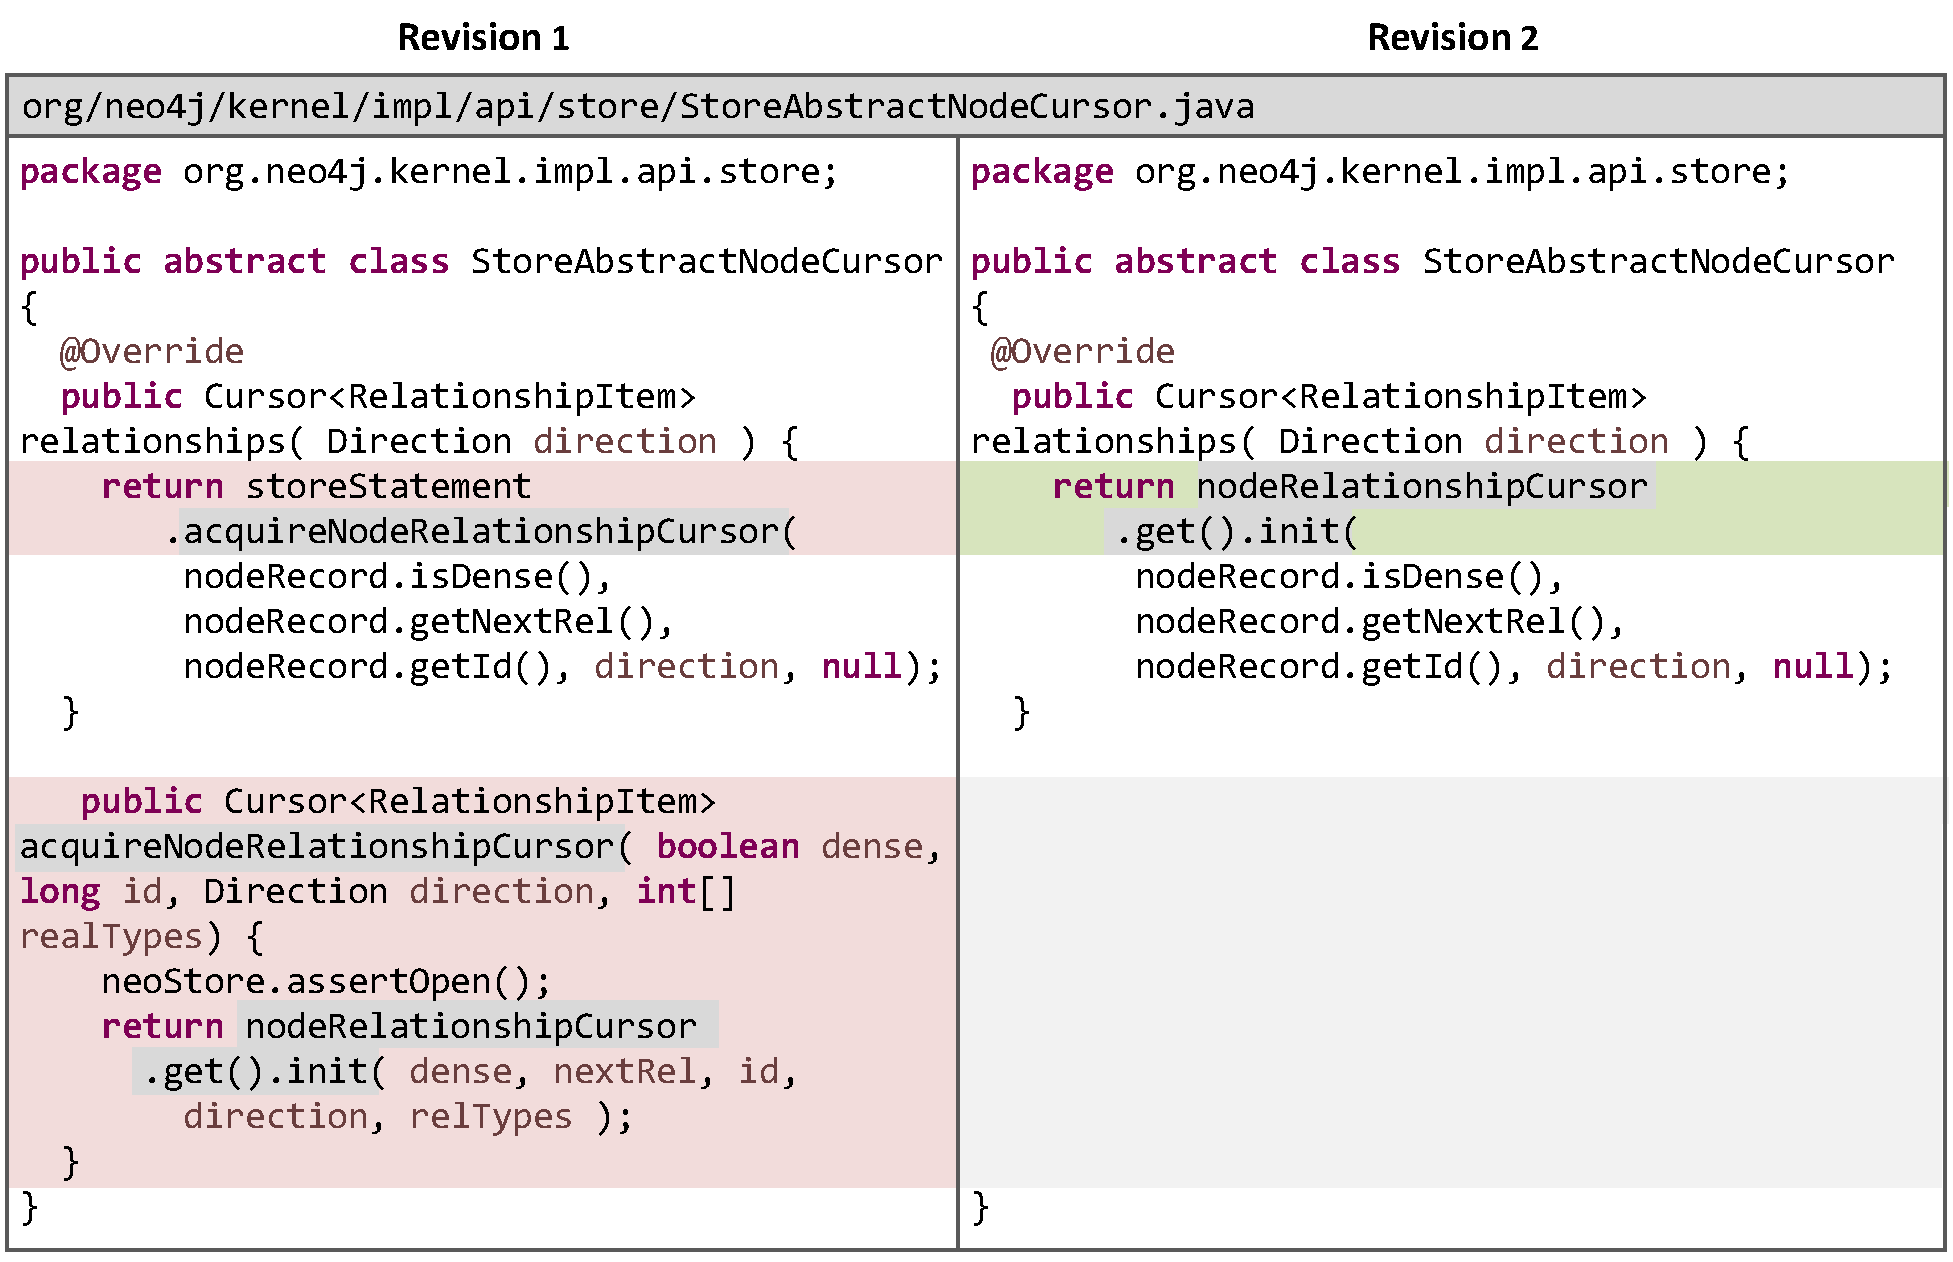
\includegraphics[width=0.8\textwidth]{img/diff2.pdf}
\caption{Illustrative diff of an \emph{Inline Method} refactoring considered as true positive by the validators.}
\label{FigDiff2}
\end{figure*}

After following this procedure, RefDiff 2.0 detected 278 new refactoring instances (i.e., not listed in the initial oracle), which were  validated by two paper's authors, called here validators. In the case of 173 refactorings (62\%), the validators agreed on their classification, including 115 refactorings labelled as true positives by both validators and 58 labelled as false positives. After this initial and independent validation, the validators discussed together the remaining 105 cases (38\%), to reach an agreement. As a result, 66 refactorings were considered true positives and 39 refactorings were classified as false positives. Figure~\ref{FigDiff2} shows a first example of true positive. RefDiff identified an \emph{Inline Method} refactoring, consisting on the substitution of the method named \codeinl{acquireNodeRelationshipCursor}, which was removed in the same commit, by invocations to methods \codeinl{get()} and \codeinl{init()}. We emphasize in this figure the changes that correspond to this refactoring. This indication of refactoring was not listed in the oracle. The validators individually analyzed this commit and both agreed that an \emph{Inline Method} was applied in this commit.



Figure~\ref{FigDiff3} shows another example of true positive, this time as an indication of \emph{Extract} and \emph{Move Method} refactorings. Developers removed the invocation to the method \codeinl{readValue(String, Class)}, which was extracted and moved to the class \codeinl{Controls}. An invocation to this new method \codeinl{validateControlsString(String)} was replaced in the same line. Similarly to the example in Figure~\ref{FigDiff2}, both validators agreed that \emph{Extract} and \emph{Move Method} were applied in this commit.

\begin{figure*}[htb]
\centering
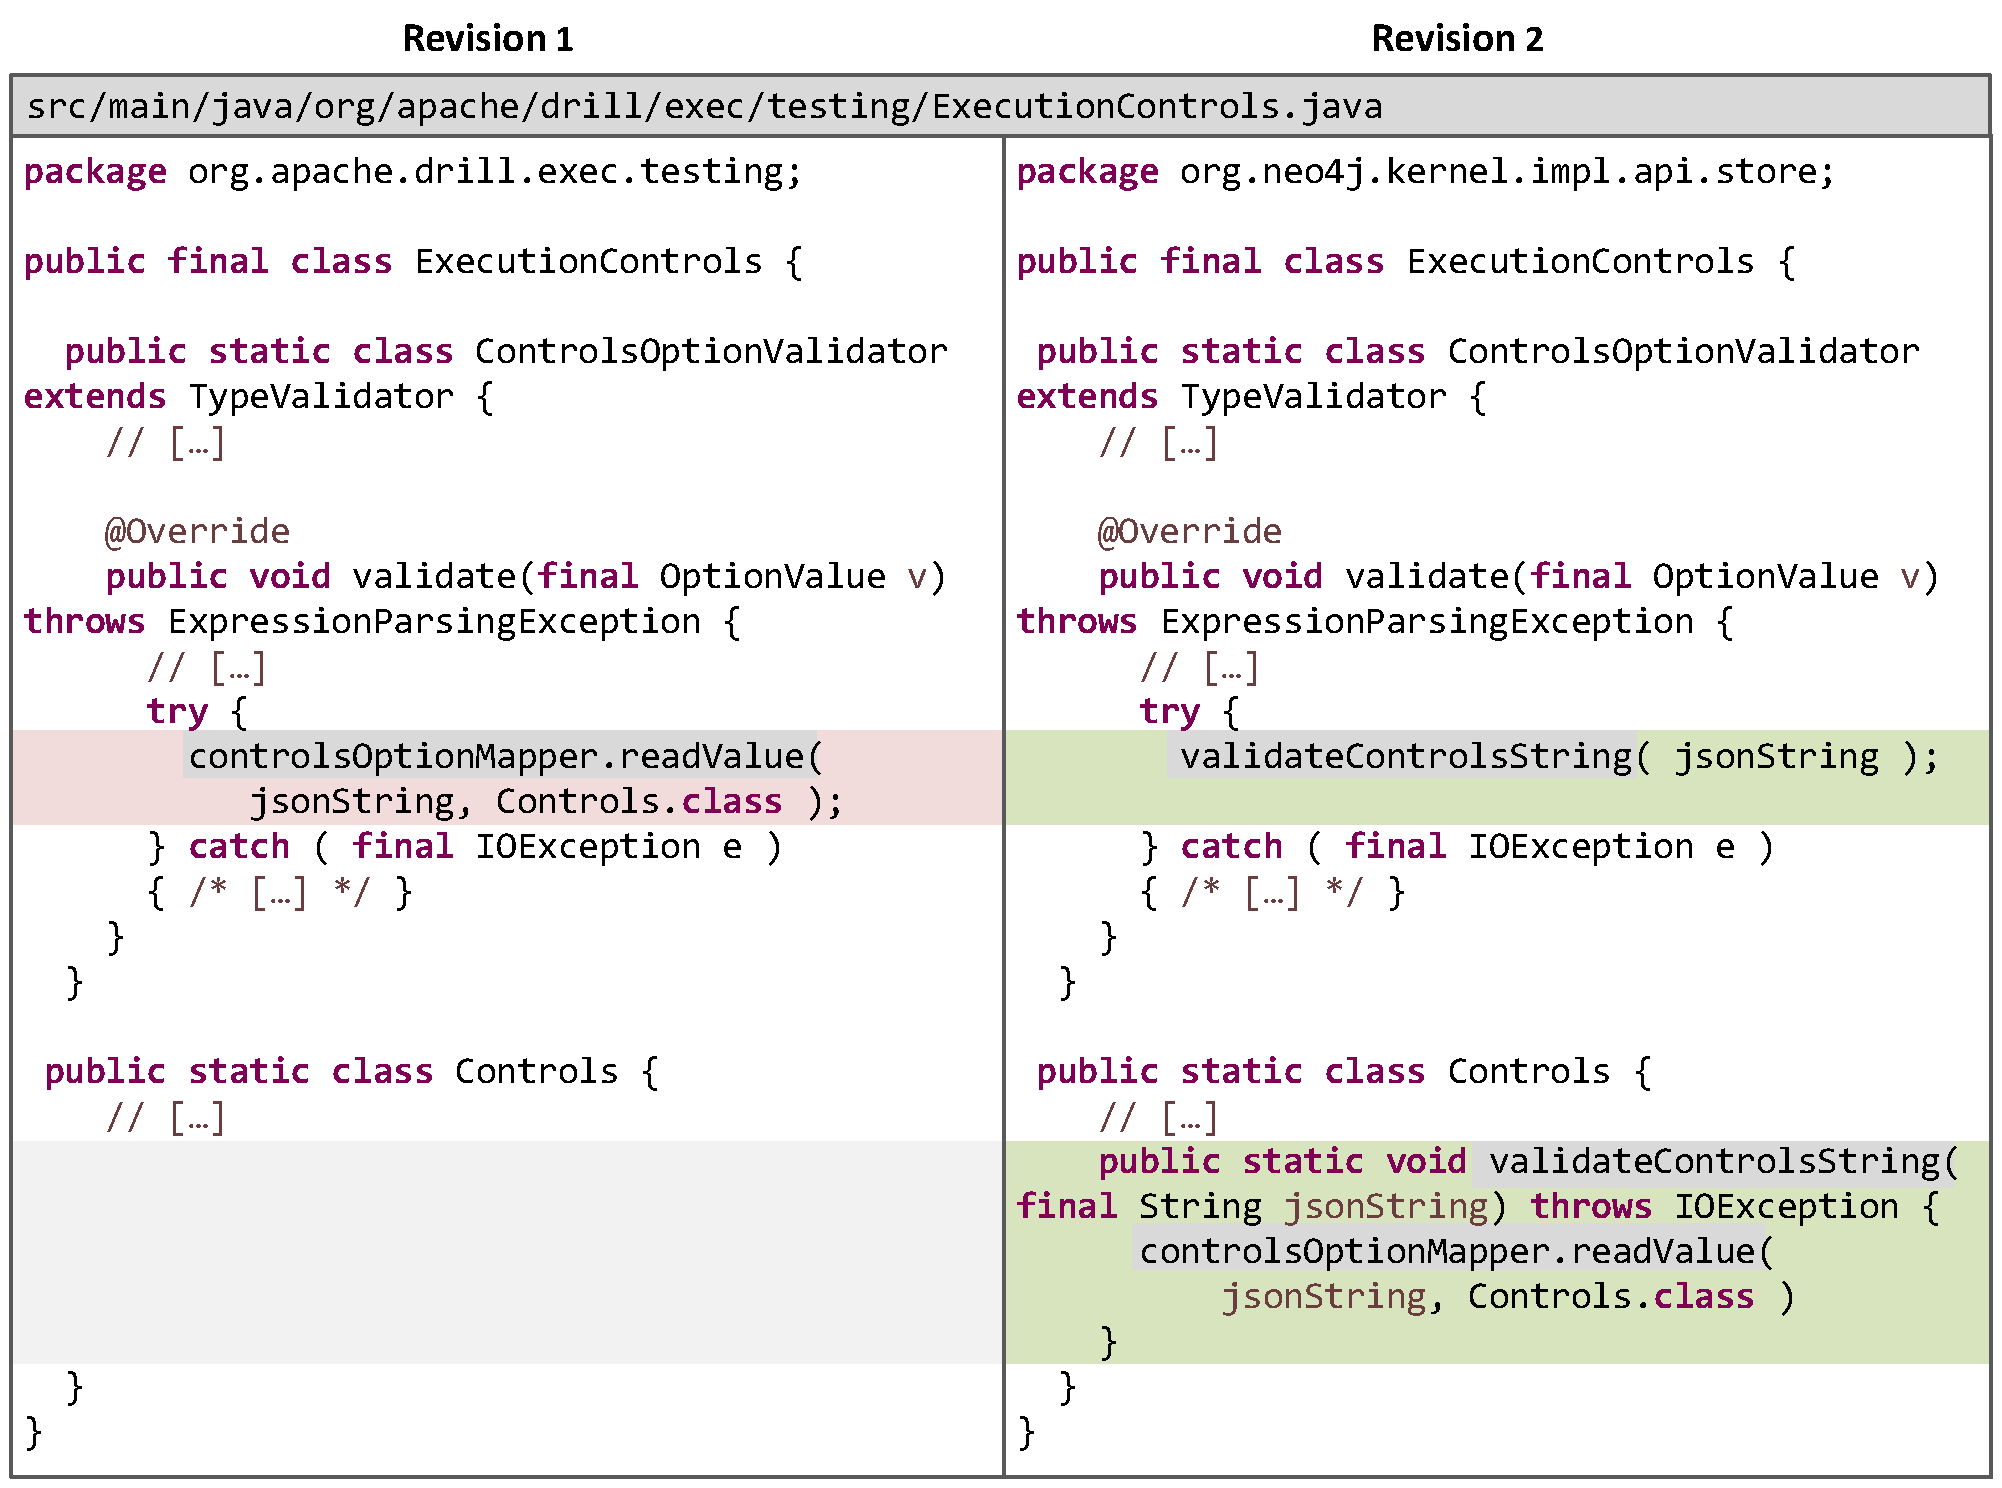
\includegraphics[width=0.8\textwidth]{img/diff3.pdf}
\caption{Illustrative diff of an \emph{Extract Method} refactoring considered as true positive by the validators.}
\label{FigDiff3}
\end{figure*}

After the manual validation of the refactoring instances it was possible to identify some common causes of failure.
In particular, one common reason for \emph{Move Method} false positives was missed \emph{Move/Rename Class}, i.e., RefDiff did not detect that the entire class has been moved (or renamed), and incorrectly reported that several of its members were moved.
We mitigated this issue by introducing a specific heuristic for this case (see Section~\ref{AlgoGeneral}).
Moreover, the analysis of the incorrect reports allowed us to identify and fix a couple of bugs in our implementation.
After applying the aforementioned fixes to RefDiff, it was necessary to run it again and compare the results against the update oracle. This time, 51 new refactoring instances were found, which were  validated by one of the authors. 24 of them (47\%) were classified as true positive, whilst 27 of them (53\%) were classified as false positive.

In summary, after these two rounds of manual validation, 184 new refactorings instances were classified as true positives and therefore included in the oracle.
The expanded oracle includes 3,261 refactoring instances (5.98\% more than the initial one) and it is publicly available at RefDiff's GitHub repository.\footnote{\url{https://github.com/aserg-ufmg/RefDiff}}

\subsection{Results}
\label{sec:eval:java:results}

\begin{table*}[htbp]
\renewcommand{\arraystretch}{1.2}
\caption{Java precision and recall results}
\label{TabResultJava}
\centering
\begin{tabular}{@{}lrlrrrlllrrrll@{}}
\toprule
 & & & \multicolumn{5}{c}{RefDiff} & & \multicolumn{5}{c}{Refactoring Miner}\\
\cmidrule{4-8} \cmidrule{10-14}
Refactoring Type & \# & & TP & FP & FN & Precision & Recall & & TP & FP & FN & Precision & Recall \\
\midrule
Move Class & 1121 & & 1067 & 1 & 54 & \xbar{0.999} & \xbar{0.952} & & 1017 & 0 & 104 & \xbar{1.000} & \xbar{0.907} \\
Move Method & 320 & & 256 & 38 & 64 & \xbar{0.871} & \xbar{0.800} & & 210 & 10 & 110 & \xbar{0.955} & \xbar{0.656} \\
Move and Rename/Rename Class & 92 & & 80 & 10 & 12 & \xbar{0.889} & \xbar{0.870} & & 59 & 1 & 33 & \xbar{0.983} & \xbar{0.641} \\
Rename Method & 346 & & 238 & 19 & 108 & \xbar{0.926} & \xbar{0.688} & & 270 & 6 & 76 & \xbar{0.978} & \xbar{0.780} \\
Extract Interface & 24 & & 21 & 3 & 3 & \xbar{0.875} & \xbar{0.875} & & 20 & 0 & 4 & \xbar{1.000} & \xbar{0.833} \\
Extract Superclass & 70 & & 52 & 0 & 18 & \xbar{1.000} & \xbar{0.743} & & 68 & 3 & 2 & \xbar{0.958} & \xbar{0.971} \\
Pull Up Method & 91 & & 75 & 2 & 16 & \xbar{0.974} & \xbar{0.824} & & 72 & 0 & 19 & \xbar{1.000} & \xbar{0.791} \\
Push Down Method & 40 & & 38 & 2 & 2 & \xbar{0.950} & \xbar{0.950} & & 33 & 0 & 7 & \xbar{1.000} & \xbar{0.825} \\
Extract/Extract and Move Method & 1037 & & 686 & 29 & 351 & \xbar{0.959} & \xbar{0.662} & & 796 & 12 & 241 & \xbar{0.985} & \xbar{0.768} \\
Inline Method & 120 & & 86 & 6 & 34 & \xbar{0.935} & \xbar{0.717} & & 97 & 1 & 23 & \xbar{0.990} & \xbar{0.808} \\
\addlinespace
Total & 3261 & & 2599 & 110 & 662 & \xbar{0.959} & \xbar{0.797} & & 2642 & 33 & 619 & \xbar{0.988} & \xbar{0.810} \\
\bottomrule
\end{tabular}
\end{table*}

Table~\ref{TabResultJava} shows the precision and recall results for RefDiff and RMiner using the oracle described in the previous section. The overall precision and recall of RefDiff is 95.9\% and 79.7\%, respectively.
Precision ranges from 87.1\% (\emph{Move Method}) to 100.0\% (\emph{Extract Superclass}), and it is above 90\% for 7 of the 10 refactoring types.
Recall ranges from 66.2\% (\emph{Extract Method}) to 95.2\% (\emph{Move Class}), and it is above 80\% for 6 of the 10 refactoring types.
On its turn, RMiner achieves 98.8\% of overall precision (ranging from 95.5\% to 100.0\%) and 81.0\% of overall recall (ranging from 64.1\% to 97.1\%).
When we analyze individual refactoring types, RefDiff's precision is always lower, but recall is higher in 6 refactoring types.
Thus, we conclude that both tools have very similar recall, but RMiner's precision is consistently higher.
Nevertheless, we argue that RefDiff's precision of 95.9\% is satisfactory, specially when we consider that our approach is programming language neutral.




